\chapter{VAR-Tool}
\label{ch:main-matter}
  \begin{figure}[H]
    \centering
    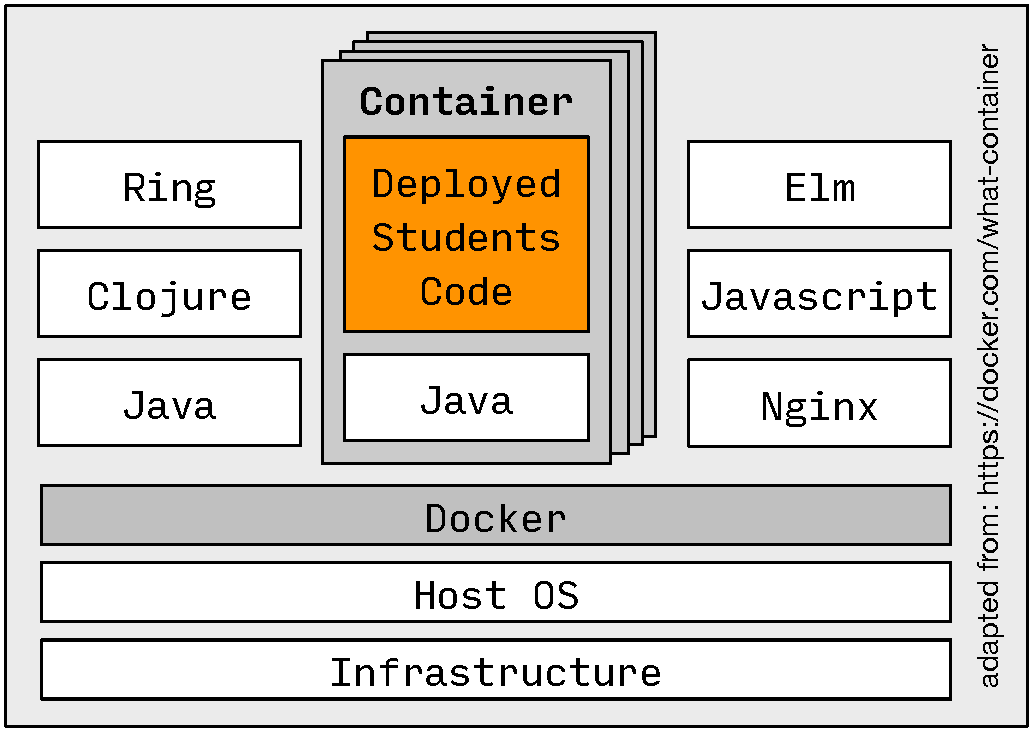
\includegraphics[scale=0.4]{container_intro_centered.pdf}
    \par
    \caption{Container-Übersicht}
    \label{fig:container-intro}
  \end{figure}
  \blindtext
  \clearpage

% \section{Analyse}
% \subsection{As-Is}
% \subsection{To-Be}

\section{UI-Mockup}
\blindtext
\begin{landscape}
  \begin{figure}[h]
    \centering
    \fbox{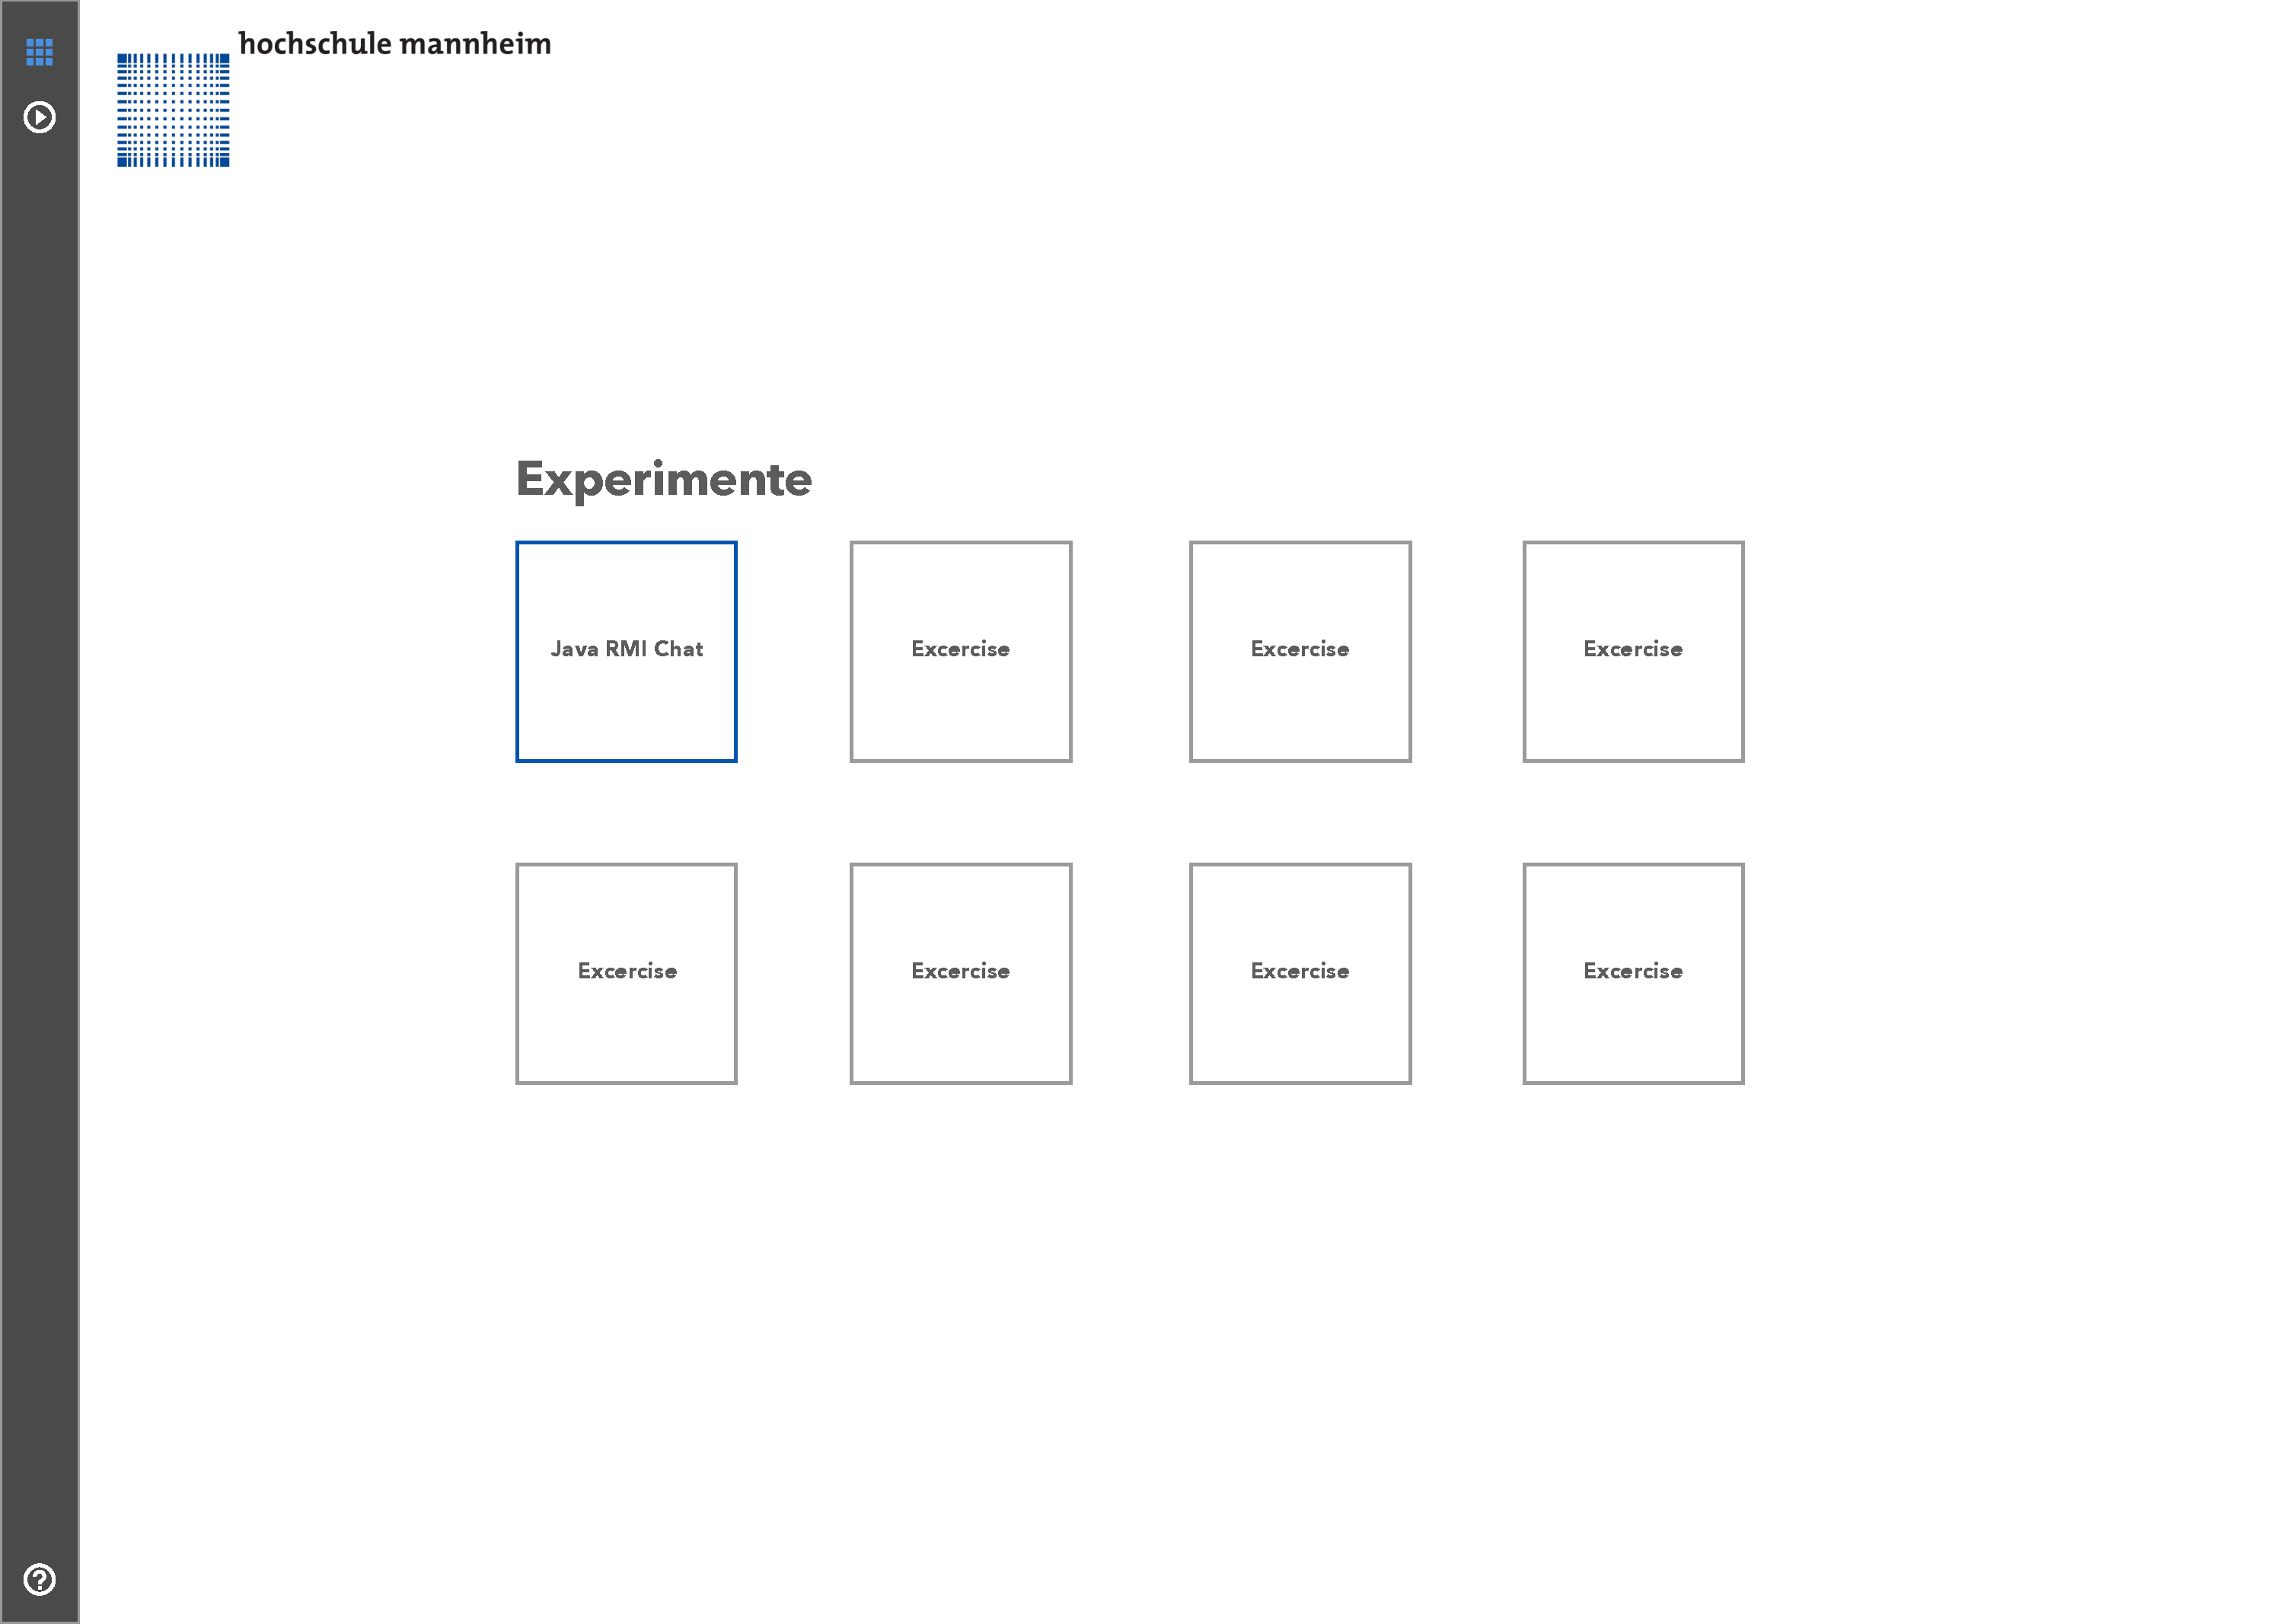
\includegraphics[scale=0.4,page=1]{ui-mockup.pdf}}
    \par
    \caption{UI-Mockup: Übersicht der Experimente}
    \label{fig:ui-mockup-1}
  \end{figure}
  \begin{figure}[h]
    \centering
    \fbox{\includegraphics[scale=0.4,page=2]{ui-mockup.pdf}}
    \par
    \caption{UI-Mockup: Experimentenansicht mit verschiedenen Zuständen pro Instanz}
    \label{fig:ui-mockup-2}
  \end{figure}
\end{landscape}
\section{Architektur}
\blindtext
\subsection{Geschäftsprozesse}
\blindtext
\begin{landscape}
  \begin{figure}[h]
    \centering
    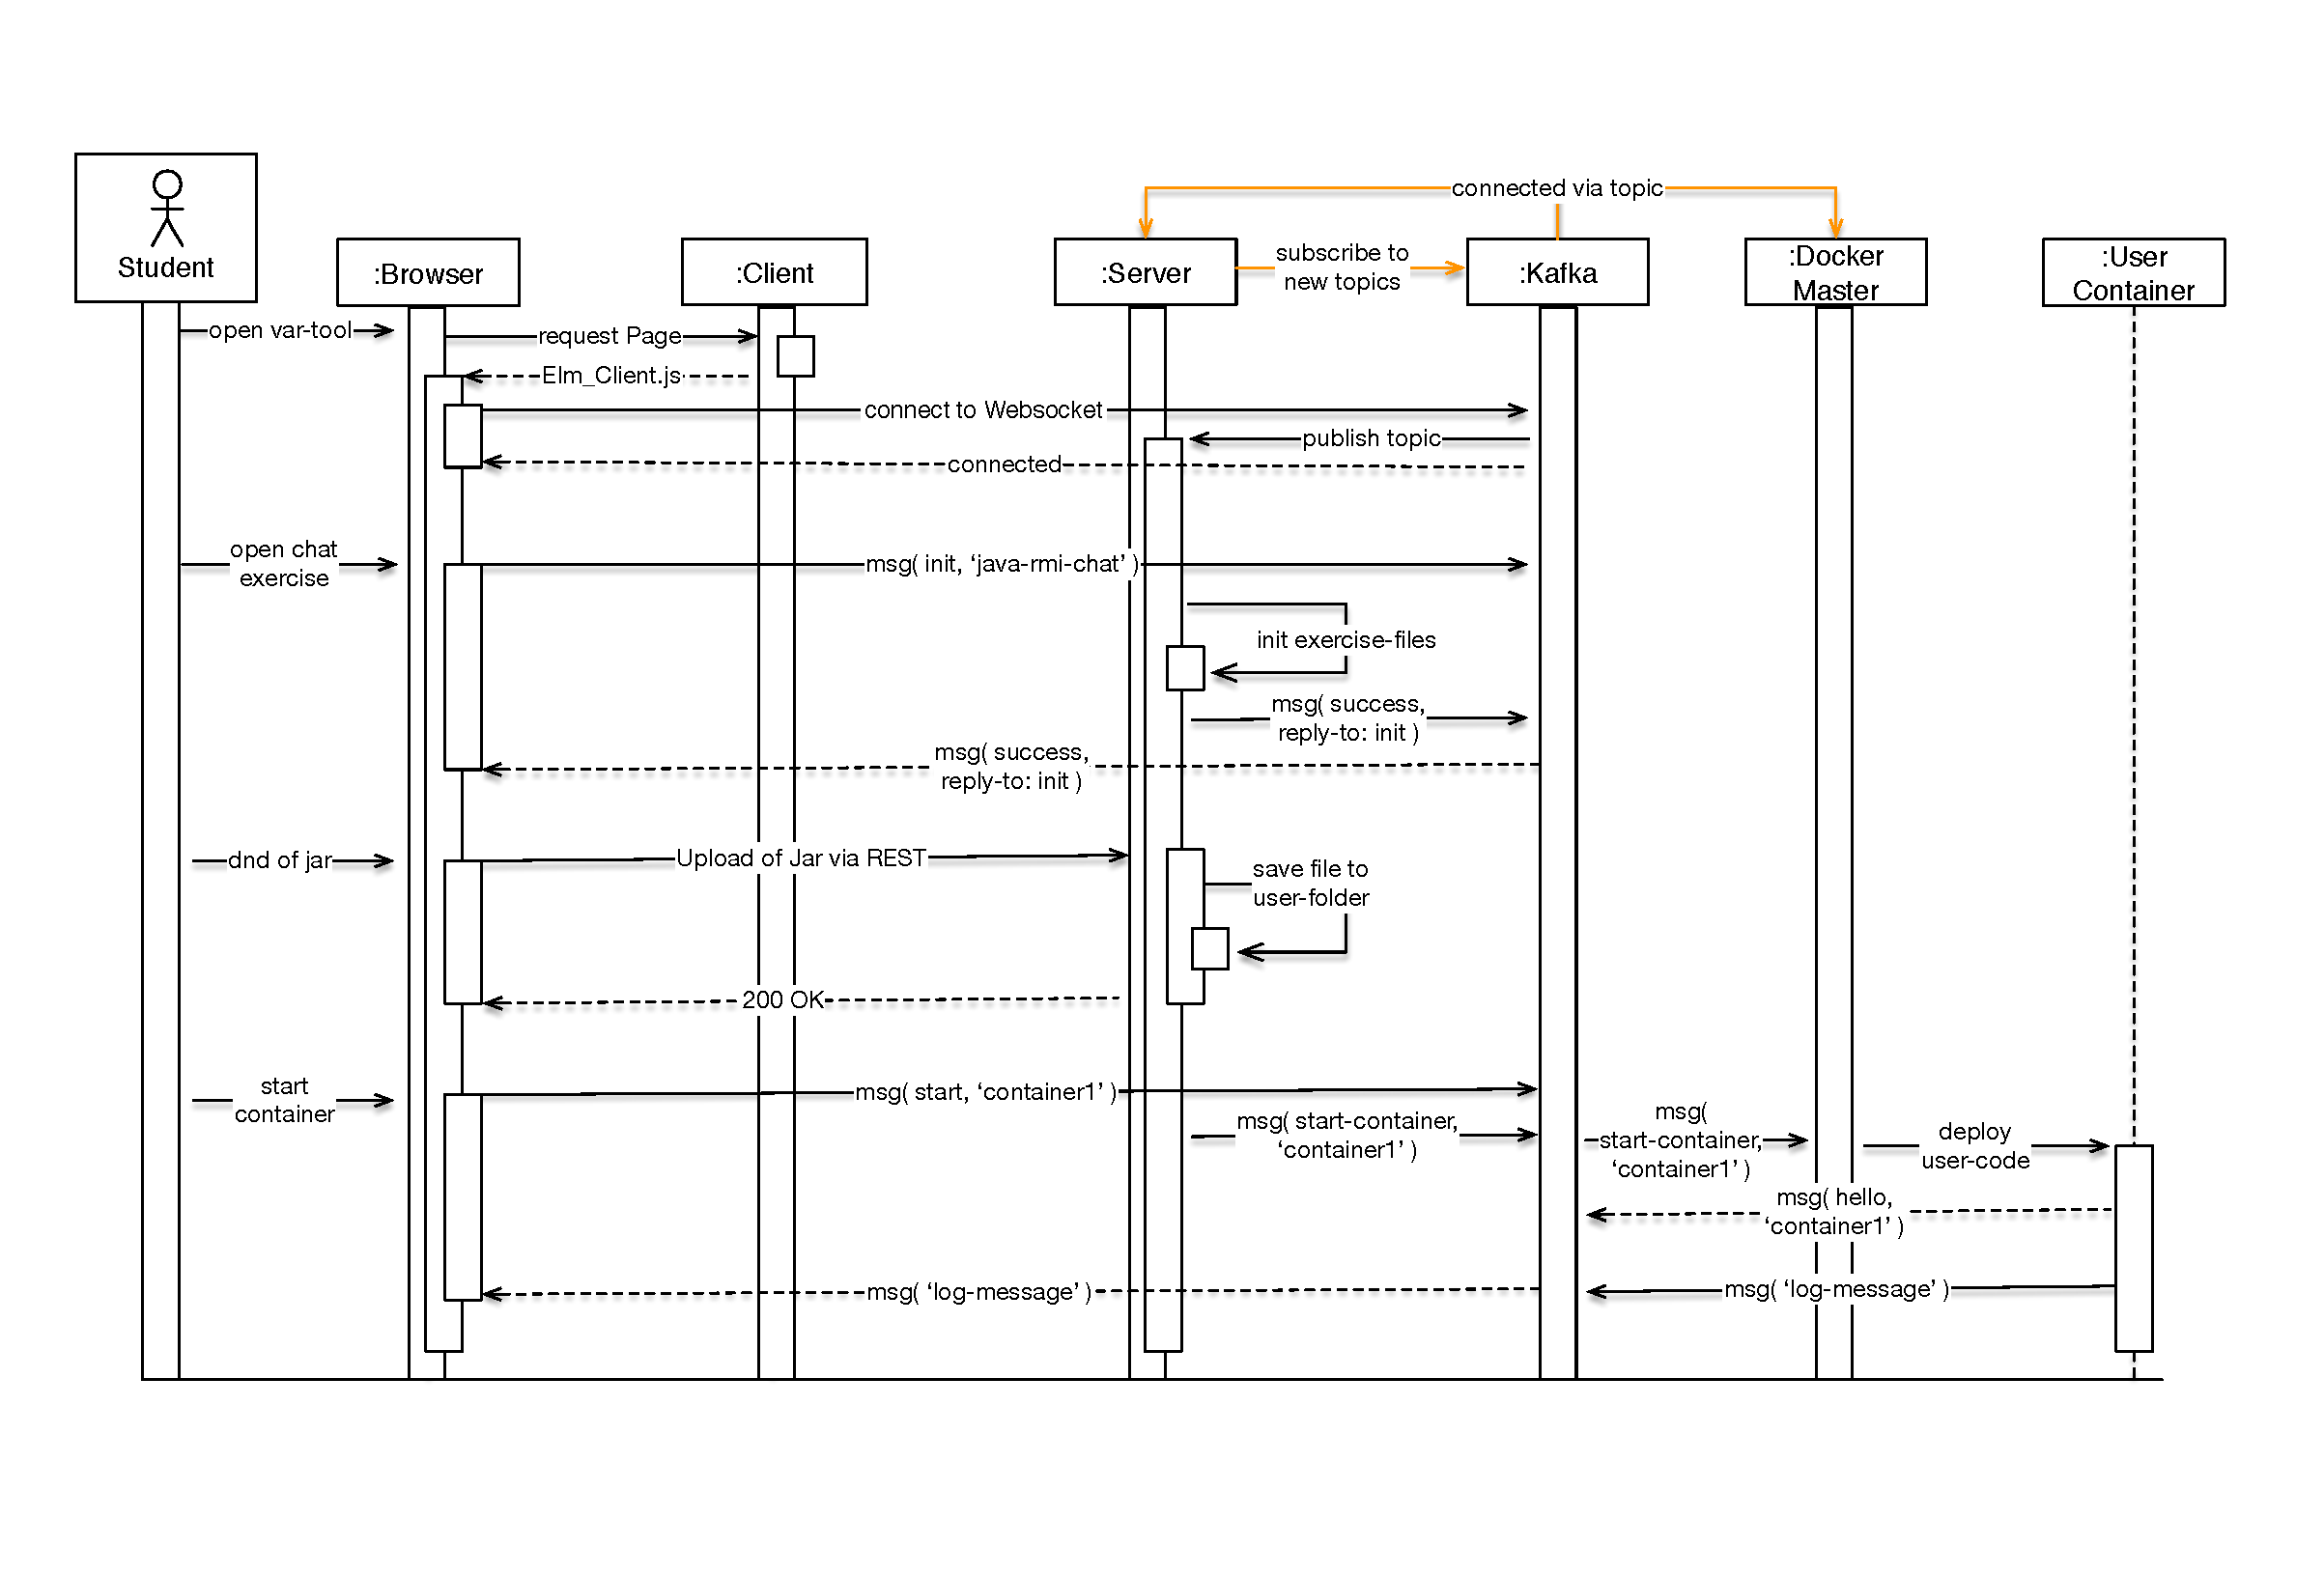
\includegraphics[scale=0.5]{sequence.pdf}
    \par
    \caption{Sequenzdiagramm}
    \label{fig:sequence}
  \end{figure}
\end{landscape}
\subsection{Netzwerkgrenzen}
\blindtext
  \begin{figure}[h]
    \centering
    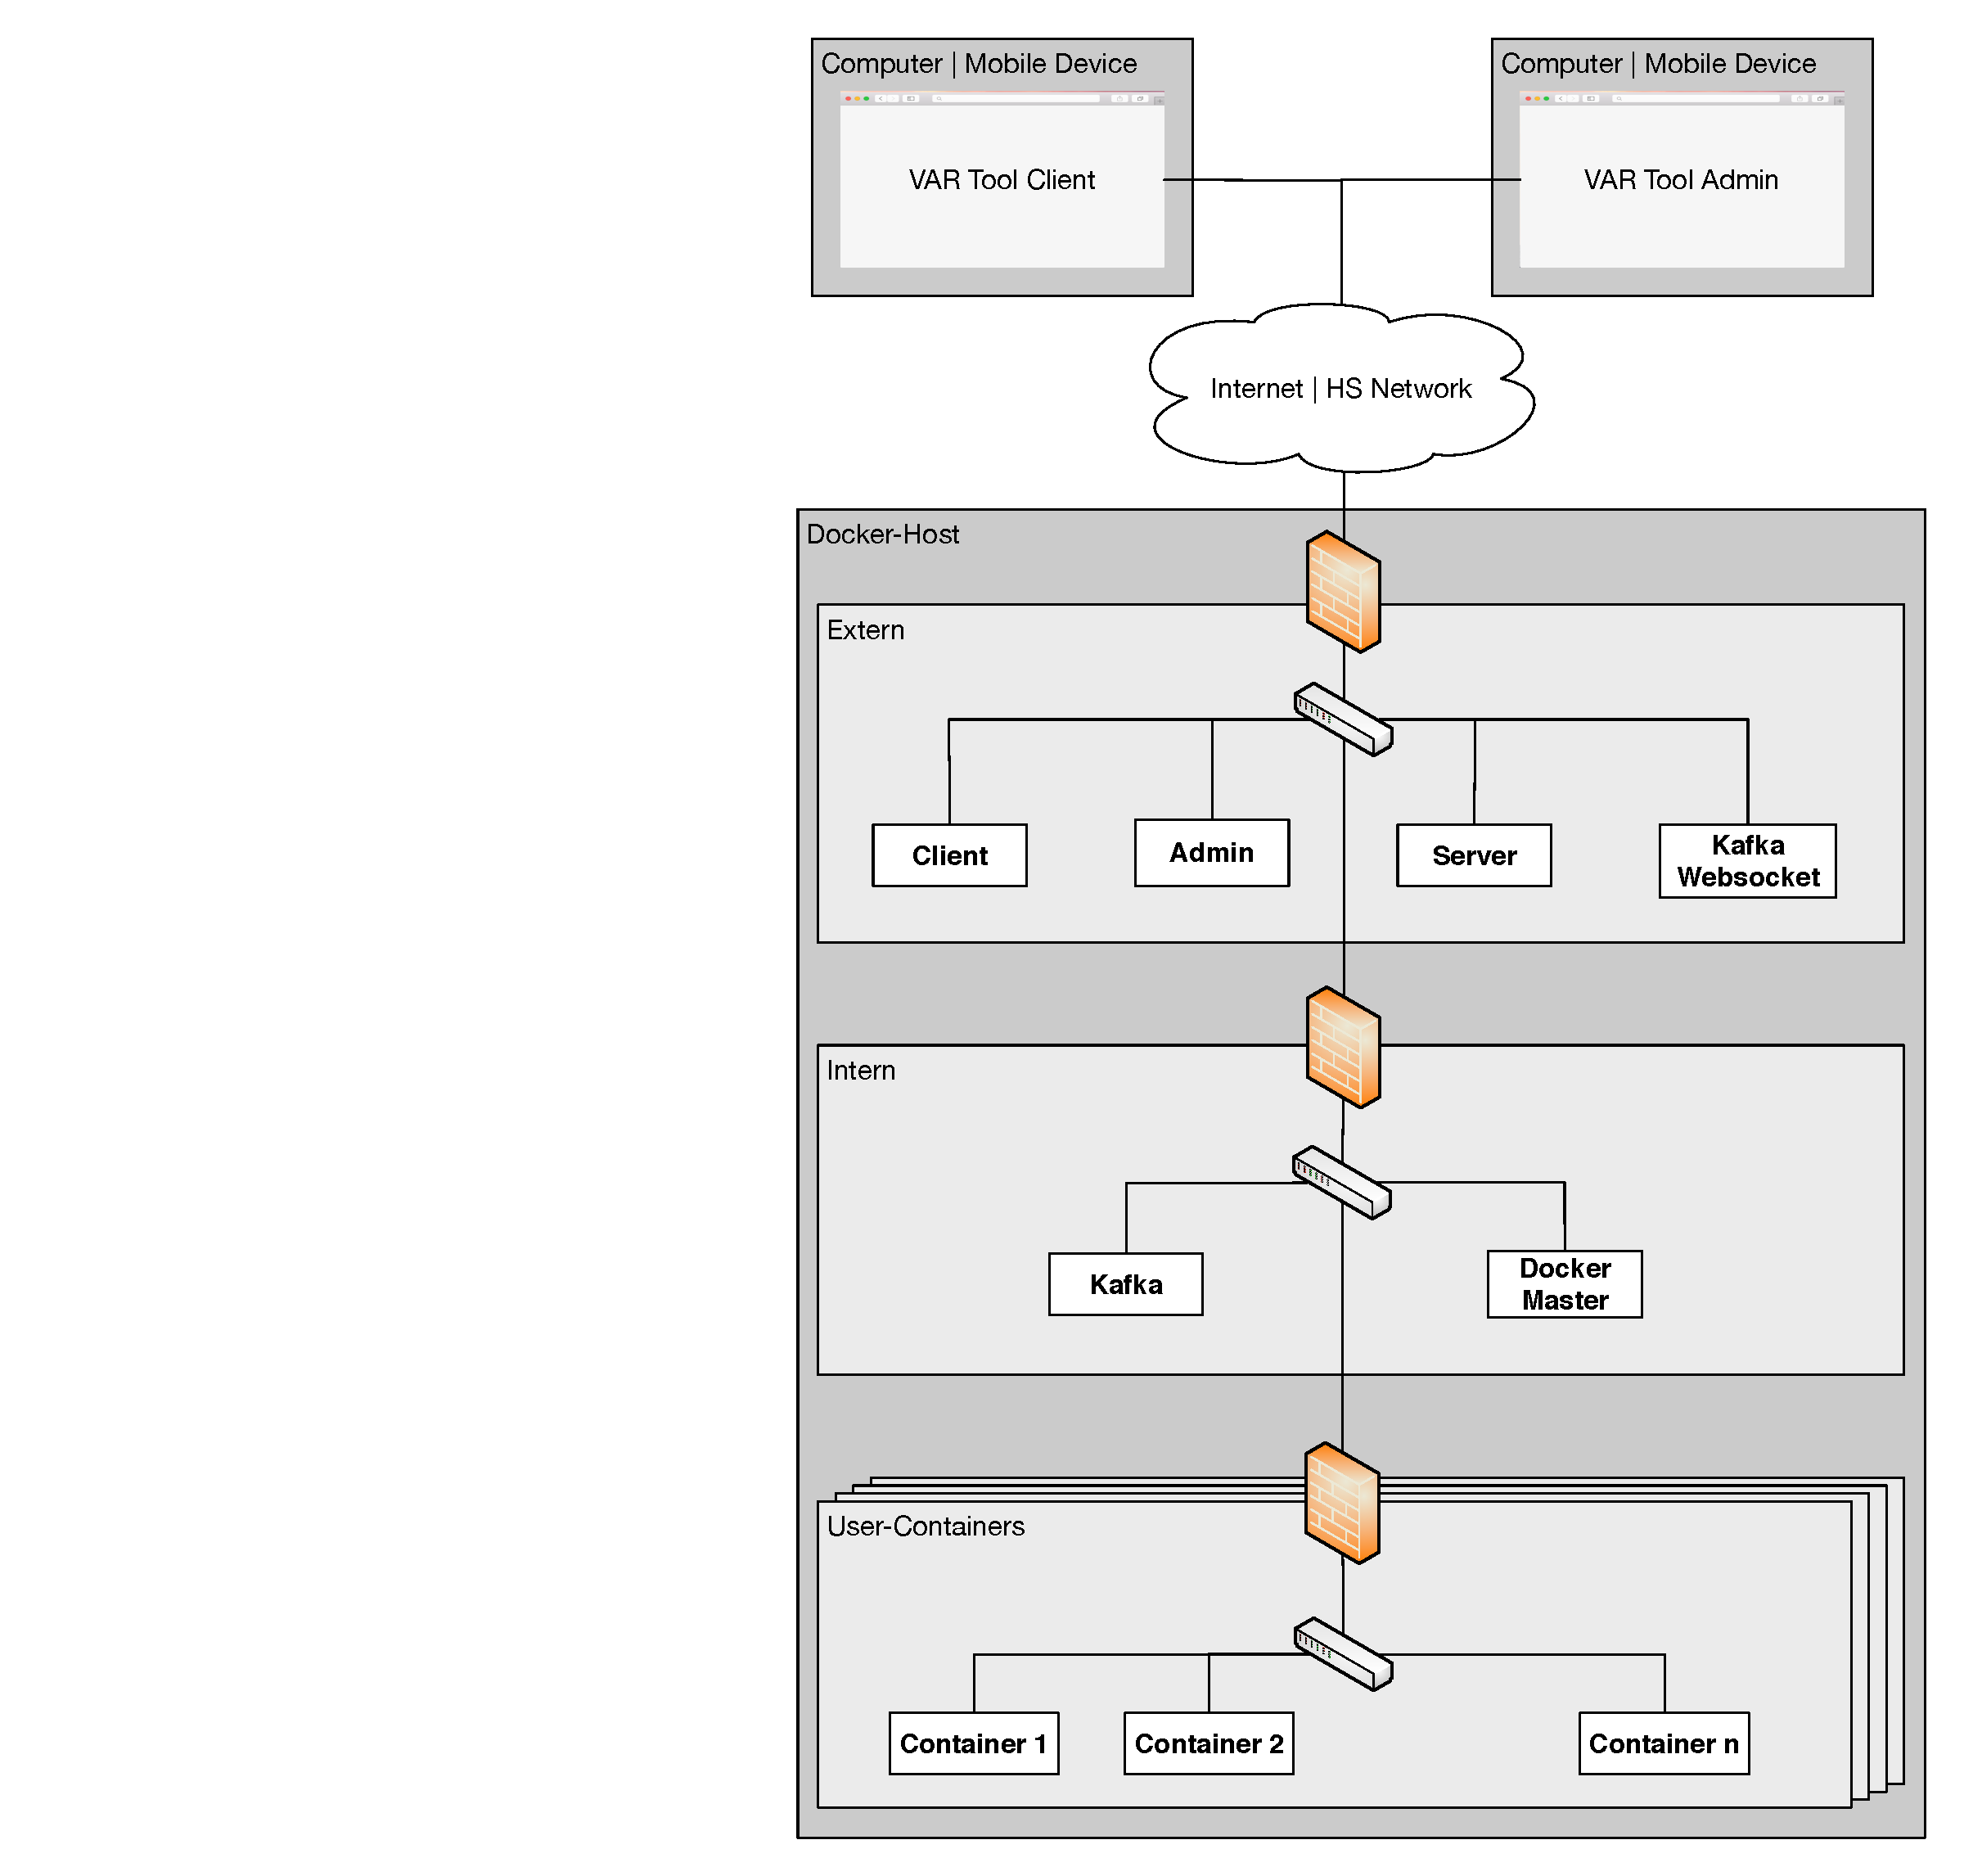
\includegraphics[scale=0.5]{network.pdf}
    \par
    \caption{Netzwerkdiagramm}
    \label{fig:network}
  \end{figure}
\subsection{Deployment}
\blindtext
\begin{landscape}
  \begin{figure}[h]
    \centering
    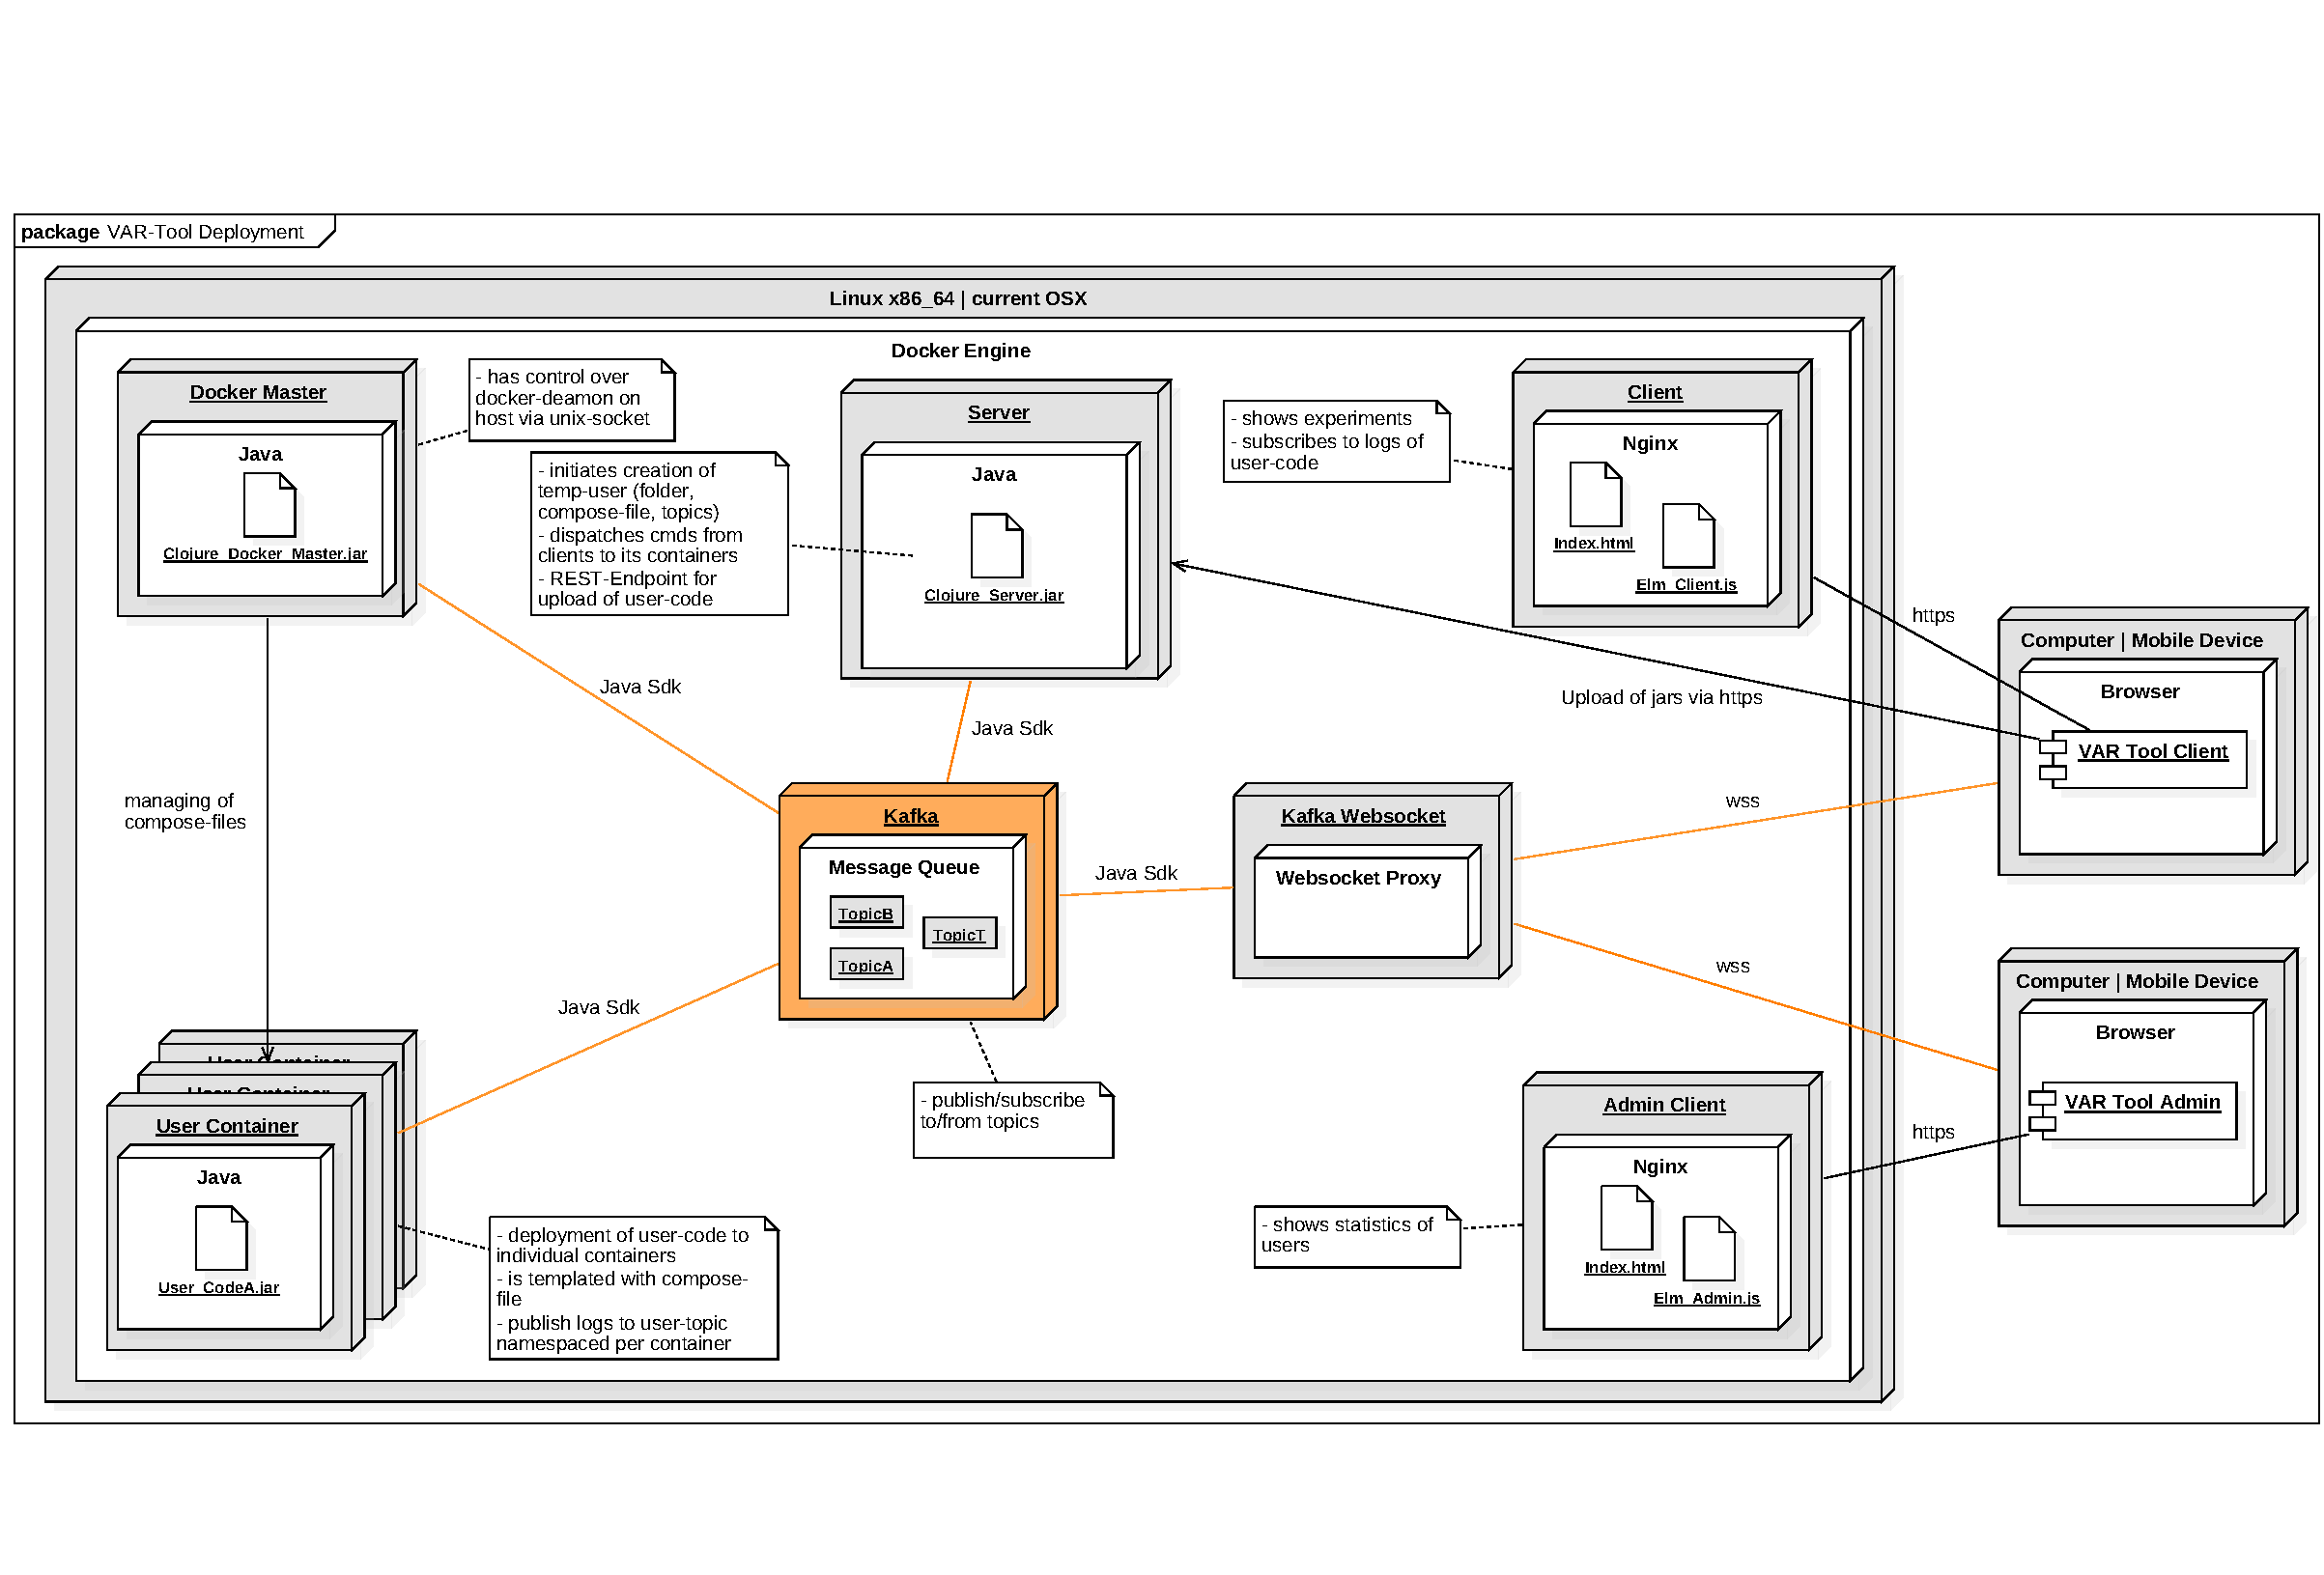
\includegraphics[scale=0.5]{deployment.pdf}
    \par
    \caption{Deploymentdiagramm}
    \label{fig:deployment}
  \end{figure}
\end{landscape}
\section{Umsetzung}
\subsection{Kommunikation über Nachrichten}
Im Vorfeld wurde ein Nachrichten-Protokoll definiert, welches die Kommunikation zwischen Server und Client standardisiert.
Dabei heißen Client-Nachrichten \textit{Commands} und Server-Nachrichten \textit{Messages}.
So können beide Nachrichten-Typen durch ein triviales Merkmal unterschieden werden.
Jeweilig unterscheiden sich diese weiter in Kinder-Typen und deren \textit{Payloads}.
Dabei werden die Daten über eine Websocket-Verbindung in einem JSON-Envelope als String übertragen.
\\\\
\textbf{Commands:}
\begin{itemize}
  \item request-experiments:
  \item add-input:
  \item start-instance:
  \item stop-instance:
\end{itemize}
\textbf{Messages:}
\begin{itemize}
  \item log:
  \item reply:
\end{itemize}

\subsection{Server}
\blindtext
\blindtext
\blindtext
\subsection{Client}
\blindtext
\blindtext
\blindtext
\section{Erwartungen an die Performance}
\section{Installation}
Als erstes wird das Projekt mithilfe von \texttt{git clone \url{https://github.com/jwillem/var-tool.git}} heruntergeladen.
Um die Applikation zu starten, werden zunächst die Installationen von Docker\footnote{\url{https://www.docker.com/community-edition}} und Docker-Compose\footnote{\url{https://docs.docker.com/compose/install/}} benötigt.
Nach einem Ausführen von \texttt{docker-compose build} im Projektverzeichnis kann die App mit \texttt{docker-compose up} gestartet werden.
